% ----------------------------------------------------------------------
% Author: Nello Blaser, ISPM, Uni Bern
%         <nblaser@ispm.unibe.ch>
% ----------------------------------------------------------------------
% Last modified: 24.07.2014
% ----------------------------------------------------------------------
% use:
%%% setwd("C:/Users/nblaser/Documents/Cohort Model/JSS manuscript/sweave")
%%% Sweave("case.Rnw")
%
% Set global Sweave options:
% - use R engine;
% - do not create eps figures;
% - create pdf figures;


% Set further Sweave options:
% - use prefix.string as prefix for \includegraphics and include
%   the figure.


% This should handle the size of the figures.
% !!! NOT SURE EXACTLY HOW AND WHETHER IT WORKS !!!
\setkeys{Gin}{width=.9\textwidth}

% ----------------------------------------------------------------------
% Initialise R session for this section

% ----------------------------------------------------------------------
\section[Case study]{Case study: Transcatheter aortic valve implantation}\label{cs}

\subsection{Introduction}
Calcific aortic stenosis is a degenerative disease characterized by progressive narrowing of the aortic valve, which compromises oxygenated blood output from the heart. Medical therapy as a sole treatment option has not improved survival among patients with symptomatic severe aortic stenosis. Surgical aortic valve replacement (SAVR) is the treatment of choice and the gold standard for aortic valve disease treatment. In the presence of serious co-morbidities, and in patients considered to be at high-risk for SAVR, transcatheter aortic valve implantation (TAVI) techniques offer less-invasive treatment of valvular aortic stenosis.  Older patients who have severe calcific aortic stenosis, characterized by the presence of co-morbidities and compromised left ventricular ejection fraction, have increased risk of complications from the surgical procedure itself. These high risk patients were managed medically until catheter-based treatment TAVI was introduced in 2002. During a TAVI implantation a bio-prosthetic valve is inserted and implanted within the diseased aortic valve through a catheter. The result of increased interest in this catheter-based approach is that this less invasive procedure is now used in patients with less severe disease \citep{Pilgrim2012}.

\subsection{Statistical analysis}

The \code{tavi} data set contains data on kidney injuries, bleeding complications and the combined endpoint of stroke or death for 194 patients. The variables \code{kidney, bleeding, death} are indicator variables that show if an event has occurred; the variables \code{kidney.dur, bleeding.dur, death.dur} are the times at which the events occurred or the patients were censored. 
\begin{Schunk}
\begin{Sinput}
R>   data("tavi")
R>   head(tavi)
\end{Sinput}
\begin{Soutput}
  id kidney kidney.dur bleeding bleeding.dur death death.dur
1 P1      0        779        0          779     0       779
2 P2      0          8        1            8     0       379
3 P3      0        342        0          342     0       342
4 P4      1          3        0            3     0        36
5 P5      1          7        0            7     1       131
6 P6      0          9        1            9     0       154
\end{Soutput}
\end{Schunk}

In the following discussion, the DAG depicted in Figure~\ref{fig:taviDAG} is assumed. Since no patients experience both kidney injury and bleeding complications, we assume these events to be mutually exclusive.
\begin{figure}[htb!]
		\centering
		\setlength{\unitlength}{2mm}
		\begin{picture}(50,30)(5,0)
		
		% Stages before Switch
		\put(10, 15){\circle{7.5}}
		\put(7.8,14.8){\textbf{\tiny{TAVI}}}
		
		\put(30, 25){\circle{7.5}}
		\put(27.8,24.8){\textbf{\tiny{Kidney}}}
		\put(30, 5){\circle{7.5}}
		\put(27.5,4.8){\textbf{\tiny{Bleeding}}}
	
		\put(50, 15){\circle{7.5}}
		\put(47.8,14.8){\textbf{\tiny{Dead}}}
	
		% Transitions
		\put(13.35, 16.68){\vector(2,1){13.29}}
		\put(13.35, 13.32){\vector(2,-1){13.29}}
		
		\put(13.75, 15){\vector(1,0){32.5}}
	
		\put(33.35, 6.68){\vector(2,1){13.29}}
		\put(33.35, 23.32){\vector(2,-1){13.29}}
		\end{picture}
	
		\caption[TAVI DAG]{\label{fig:taviDAG} DAG for case study on TAVI.}
\end{figure}

We then create the transition matrix using the \pkg{mstate} package. According to the DAG the transition matrix is given by
\begin{Schunk}
\begin{Sinput}
R>   tmat <- transMat(x = list(c(2, 3, 4), c(4), c(4), c()), 
+                  names = c("TAVI", 
+                            "Kidney Injury", 
+                            "Bleeding", 
+                            "Stroke/Death"))
R>   tmat
\end{Sinput}
\begin{Soutput}
               to
from            TAVI Kidney Injury Bleeding Stroke/Death
  TAVI            NA             1        2            3
  Kidney Injury   NA            NA       NA            4
  Bleeding        NA            NA       NA            5
  Stroke/Death    NA            NA       NA           NA
\end{Soutput}
\end{Schunk}

In order to estimate the transition-specific hazard functions, we prepare the data using the \pkg{mstate} package. We use \code{msprep} to get the data into long format, and \code{split} to split the data according to the transition. 
\begin{Schunk}
\begin{Sinput}
R>   mstavi <- msprep(data = tavi, trans = tmat, 
+                  time = c(NA, "kidney.dur", "bleeding.dur", "death.dur"),
+                  status = c(NA, "kidney", "bleeding",  "death"))
R>   head(mstavi)
\end{Sinput}
\begin{Soutput}
An object of class 'msdata'

Data:
  id from to trans Tstart Tstop time status
1  1    1  2     1      0   779  779      0
2  1    1  3     2      0   779  779      0
3  1    1  4     3      0   779  779      0
4  2    1  2     1      0     8    8      0
5  2    1  3     2      0     8    8      1
6  2    1  4     3      0     8    8      0
\end{Soutput}
\begin{Sinput}
R>   mstavi$time[mstavi$time == 0] <- .Machine$double.eps
R>   msplit <- split(mstavi, mstavi$trans)
R>   head(msplit[[5]])
\end{Sinput}
\begin{Soutput}
An object of class 'msdata'

Data:
    id from to trans Tstart Tstop time status
7    2    3  4     5      8   379  371      0
22   6    3  4     5      9   154  145      0
44  13    3  4     5      7     8    1      1
84  25    3  4     5     10   154  144      0
99  29    3  4     5      6   847  841      1
103 30    3  4     5      3     8    5      1
\end{Soutput}
\end{Schunk}

As a first step we fit an exponential distribution to all transition times. For each transition, we estimate the rate and the variance. 
\begin{Schunk}
\begin{Sinput}
R>   exp.fit <- sapply(msplit, function(x) 
+     summary(survreg(Surv(time, status) ~ 1, 
+                     data = x, 
+                     dist = "exponential")))
R>   exp.coef <- unlist(exp.fit["coefficients", ])
R>   exp.var <- unlist(exp.fit["var", ])
\end{Sinput}
\end{Schunk}

Next we specify the model, simulate from it and compare the simulated mortality to a Kaplan-Meier graph of mortality.
\begin{Schunk}
\begin{Sinput}
R>   states <- 4
R>   maxtime <- max(mstavi$time)
R>   ind <- which(!is.na(tmat), arr.ind = TRUE)
R>   hm <- generateHazardMatrix(states)
R>   for (i in 1:dim(ind)[1]){
+     hm[[ind[i, 1], ind[i, 2]]] <- "Weibull"
+   }
R>   par <- generateParameterMatrix(hm)
R>   for (i in 1:dim(ind)[1]){
+     par[[ind[i, 1], ind[i, 2]]] <- list(shape = 1, 
+                                         scale = exp(exp.coef[i]))
+   }
R>   cov <- generateParameterCovarianceMatrix(par)
R>   for (i in 1:dim(ind)[1]){
+     cov[[ind[i, 1], ind[i, 2]]] <- matrix(c(0, 0, 0, exp.var[i]), nrow=2)
+   }
R>   ds <- simulateCohort(transitionFunctions = hm, 
+                       parameters = par, 
+                       cohortSize = 100 * nrow(tavi), 
+                       parameterCovariances = cov,
+                       to = maxtime)
R>   cinc <- cumulativeIncidence(ds, 0:maxtime, colnames(tmat), M = 100)
\end{Sinput}
\end{Schunk}

%<<expPlot,include=FALSE>>=
%  plot(survfit( Surv(death.dur, death)~1, 
%                data=tavi), 
%       fun="event", xlim=c(0,maxtime), ylim=c(0,1), lwd=2)
%  lines(survfit( Surv(toD, soD)~1), fun="event", col=2, lwd=2)
%  legend(200, .8, c("Data", "Simulation"), lty=1, col=1:2, lwd=2)
%@
%
%\begin{figure}
%\begin{center}
%<<label=expPlot,fig=TRUE,echo=FALSE>>=
%<<expPlot>>
%@
%\end{center}
%\caption{Kaplan-Meier of the data and exponential simulation}
%\label{fig:expPlot}
%\end{figure}

Figure~\ref{fig:PWexpPlot} shows the overall mortality from the simulated cohort. 
Because the purpose of this study is to illustrate the use and flexibility of the package, we split time into monthly intervals and calculate piecewise constant hazard functions using the \code{pehaz} function from the \pkg{muhaz} package. 
%If the aim was to study TAVI in more detail,  we would instead consider each transition separately, and fit an appropriate parametric distribution.

\begin{Schunk}
\begin{Sinput}
R>   timeStep <- 30
R>   pwexp <- sapply(msplit, function(x) pehaz(x$time,
+                                             x$status,
+                                             width = timeStep, 
+                                             min.time = 0,
+                                             max.time = max(mstavi$time)))
R>   cuts <- pwexp["Cuts", ]
R>   pwhazard <- pwexp["Hazard", ]
\end{Sinput}
\end{Schunk}

We parameterize the hazard functions with piecewise constant hazards and simulate again.
\begin{Schunk}
\begin{Sinput}
R>   hm2 <- generateHazardMatrix(states)
R>   for (i in 1:dim(ind)[1]){
+     hm2[[ind[i, 1], ind[i, 2]]] <- function(t, rates) {
+       rates[t / timeStep + 1]
+     }
+   }
R>   par2 <- generateParameterMatrix(hm2)
R>   for (i in 1:dim(ind)[1]){
+     par2[[ind[i, 1], ind[i, 2]]] <- list(rates = pwhazard[[i]])
+   }
R>   ds2 <- simulateCohort(transitionFunctions = hm2, 
+                         parameters = par2, 
+                         cohortSize = 100 * nrow(tavi), 
+                         to = maxtime)
R>   cinc2 <- cumulativeIncidence(ds2, 0:maxtime, colnames(tmat), M = 100)
\end{Sinput}
\end{Schunk}

The plot function also admits an argument \code{states}, which can be used in order to only \code{plot} certain states as shown in the following example. 
\begin{Schunk}
\begin{Sinput}
R>   plot(cinc, states = 4, axes = FALSE, frame = TRUE, col = 2, 
+        xlab = "Time (in months)", main = "Mortality", ci = TRUE)
R>   lines(survfit(Surv(death.dur, death) ~ 1, data = tavi), 
+         fun = "event", lwd = 2)
R>   lines(survfit( Surv(death.dur, death)~1, data=tavi), 
+         fun="event", lwd=2, conf.int=TRUE, lty=2)
R>   par(new = TRUE)
R>   plot(cinc2, states = 4, axes = FALSE, frame = TRUE, col = 3, 
+        xlab = "", main = "", ci = TRUE)
R>   axis(2); axis(4)
R>   axis(1, at = (0:13*90)[0:6*2+1], labels = (0:13*3)[0:6*2+1])
R>   legend(200, .8, c("Data", 
+                     "Simulation: exponential", 
+                     "Simulation: piecewise exponential"), 
+          lty = 1, col = c(1:3), lwd = 2)
\end{Sinput}
\end{Schunk}

\begin{figure}
\begin{center}
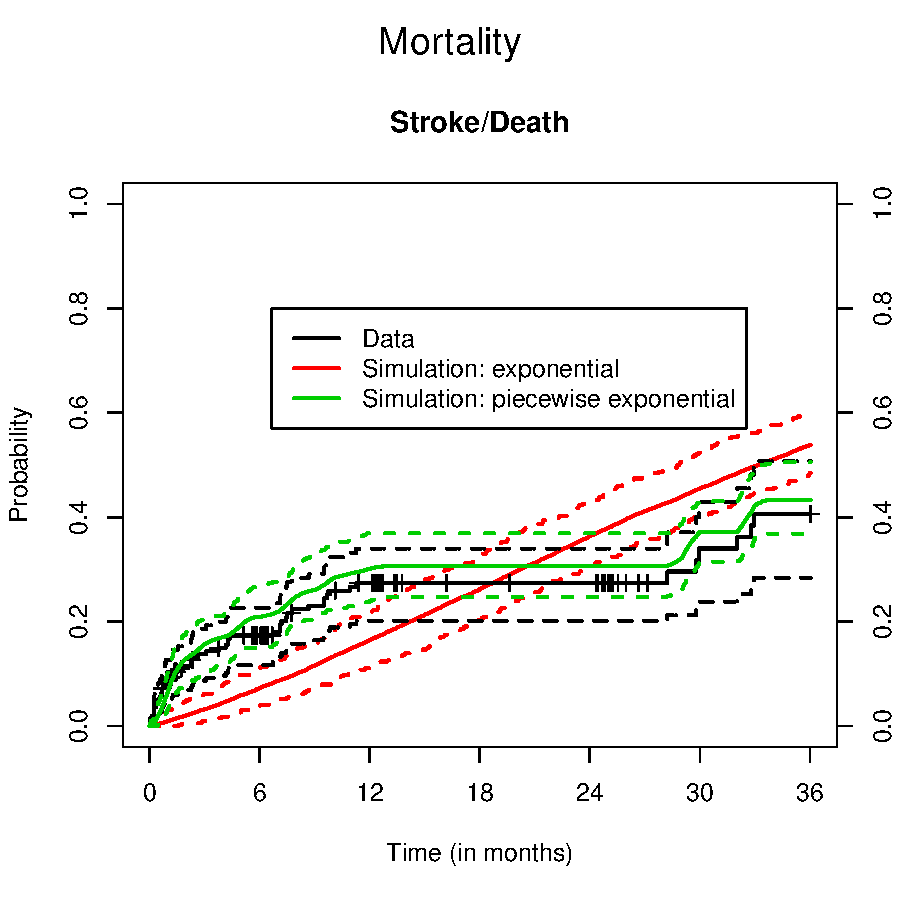
\includegraphics{PDF/Application-PWexpPlot}
\end{center}
\caption{Cumulative incidence with constant and piecewise constant transition-specific hazard functions.}
\label{fig:PWexpPlot}
\end{figure}

%The second simulation fits the data well as shown in Figure~\ref{fig:PWexpPlot}. 
%A different parametric survival function could also be used, but since we intend to demonstrate the advantages of the package \pkg{gems}, we will not elaborate on this. 
Figure~\ref{fig:PWexpPlot} shows how the simulated cumulative incidence depends on the statistical model. The package \pkg{gems} admits the choice of any transition-specific hazard function. 
We will now use the second model with piecewise constant hazard functions to estimate the effect of an intervention on mortality.
%We are now satisfied with the fit and use the model to estimate the effect of an intervention.

\subsection{Intervention modeling}
Suppose there is a new intervention that dramatically reduces the probability of getting bleeding complications, and we are interested in the impact of this intervention on mortality. 
For simplicity, we assume that the intervention reduces the transition-specific hazard of bleeding complications by $80\%$. Then 
\begin{Schunk}
\begin{Sinput}
R>   hm3 <- hm2
R>   par3 <- par2
R>   par3[[1, 3]]$rates <- par3[[1, 3]]$rates / 5
R>   ds3 <- simulateCohort(transitionFunctions = hm3, 
+                         parameters = par3, 
+                         cohortSize = 100 * nrow(tavi), 
+                         to = maxtime)
R>   cinc3 <- cumulativeIncidence(ds3, 0:maxtime, colnames(tmat), M = 100)
\end{Sinput}
\end{Schunk}

\begin{Schunk}
\begin{Sinput}
R>   plot(cinc2, states = 4, axes = FALSE, frame = TRUE, col = 1, ci = TRUE, 
+        xlab = "Time (in months)", main = "Mortality")
R>   par(new = TRUE)
R>   plot(cinc3, states = 4, axes = FALSE, frame = TRUE, col = 2, ci = TRUE, 
+        xlab = "", main = "")
R>   axis(2); axis(4)
R>   axis(1, at = (0:13 * 90)[0:6*2 + 1], labels = (0:13 * 3)[0:6 * 2 + 1])
R>   legend(200, .8, c("No intervention", "Intervention"), 
+          lty = 1, col = 1:2, lwd = 2)
\end{Sinput}
\end{Schunk}

\begin{figure}
\begin{center}
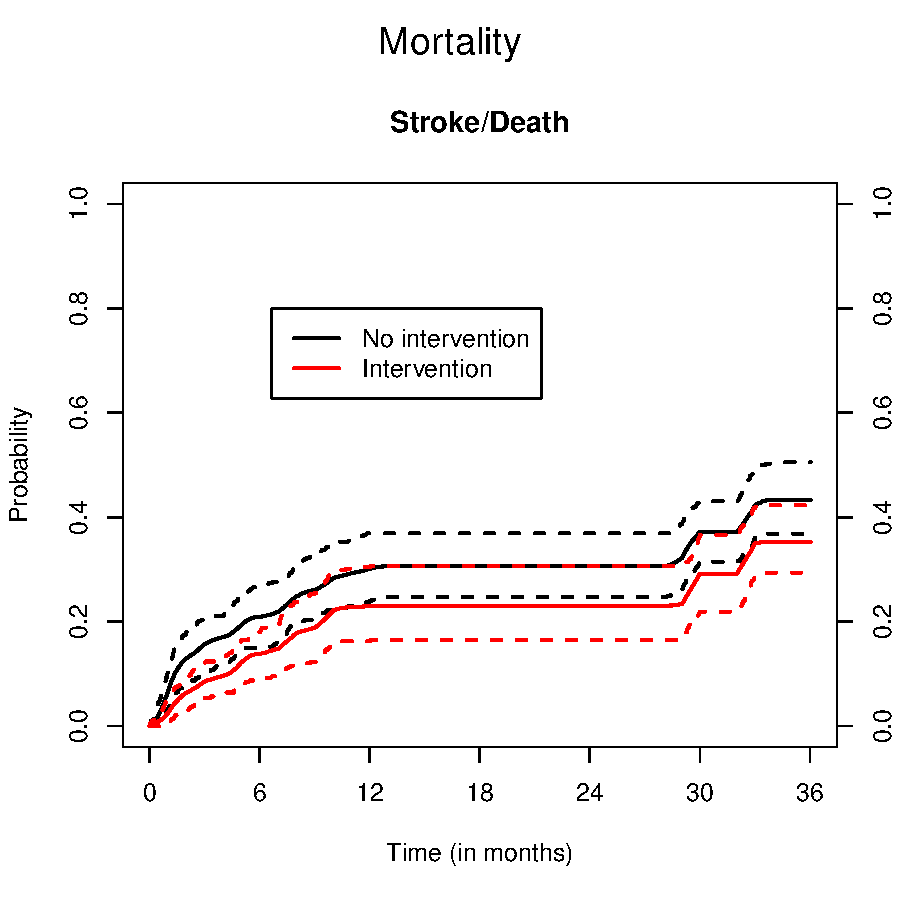
\includegraphics{PDF/Application-InterPlot}
\end{center}
\caption{Effect of reducing bleeding complications on mortality.}
\label{fig:InterPlot}
\end{figure}


Figure~\ref{fig:InterPlot} shows that reducing bleeding complications by $80\%$ decreases three-year mortality by $18.5\%$ from $43.3\%$ to $35.3\%$.
